\documentclass{beamer}
 
\usepackage[frenchb]{babel}
\usepackage[T1]{fontenc}
\usepackage[utf8]{inputenc}

 
\usetheme{Frankfurt}
  
\title{Compresseur universel}
\author{Noé LE PHILIPPE}
\institute{}
\date{\today}
% \logo{\includegraphics[height=10mm]{images/logo.png}}

\addtobeamertemplate{navigation symbols}{}{%
    \usebeamerfont{footline}%
    \usebeamercolor[fg]{footline}%
    \hspace{1em}%
    \insertframenumber/\inserttotalframenumber
}

\AtBeginSection[]
{
  \begin{frame}
  \frametitle{Sommaire}
  \tableofcontents[currentsection, hideothersubsections]
  \end{frame} 
}

\begin{document}

\begin{frame}
  \titlepage
\end{frame}

\section{Structure du compresseur}
\subsection{Compression en deux temps}
\begin{frame}
  \frametitle{Compression d'image}
  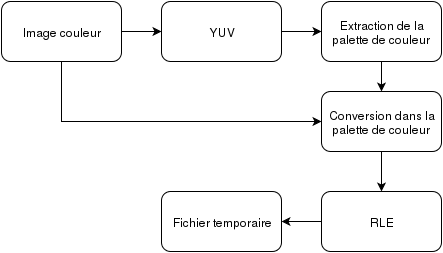
\includegraphics[scale=0.3]{image_compress.png}
  \pause
\end{frame}
\end{document}
